\section{Introduction}

The natural world is full of fascinating phenomena. Our ancestors have worked tirelessly to develop the language of mathematics to describe these phenomena. While exact analytic solutions to some of the more complicated problems often do not exist, or are too impractical to solve by hand, there are numerical techniques to approximate the solutions to these problems. However, the numerical techniques are still quite laborious to compute. Powerful institutions could employ teams of computers to labor for hours solving problems of science and engineering that we would find trivial today. 

We live in an exciting point in history where the profession of computer has been fully automated by machines. And not just automated for powerful institutions, but also made accessible to nearly all of humanity. The amount of compute accessible to anyone reading this paper is beyond the comprehension of our ancestors who originally developed the mathematics we shall employ. 

Modern hardware is capable of computing small models in what feels like an instant, and with these models we can foresee the future. As engineers, we must be comfortable wielding this immense power. 

In this paper we shall identify some physical phenomenon, develop a mathematical model of it, and develop computer software to compute the model.

\subsection{Selecting a Phenomenon}

We're interested in modeling a phenomenon which is simple enough in scope to implement over a couple weeks, but could be representative of some more complex system being used in the world today. 

\begin{figure*}[t!]
    \centering
    \begin{subfigure}[t]{0.5\textwidth}
        \centering
        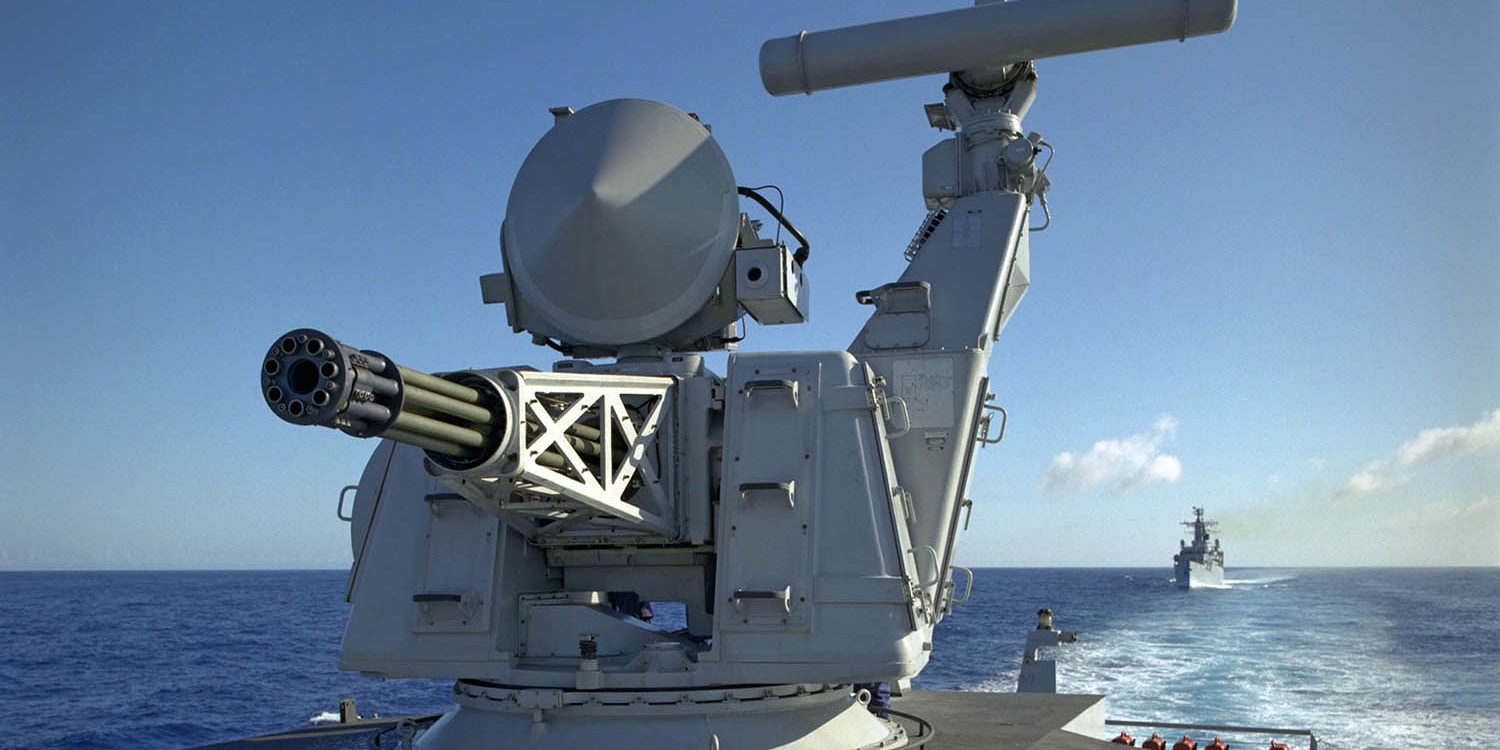
\includegraphics[height=1.5in]{images/CIWS.jpg}
        \caption{}
    \end{subfigure}%
    ~ 
    \begin{subfigure}[t]{0.5\textwidth}
        \centering
        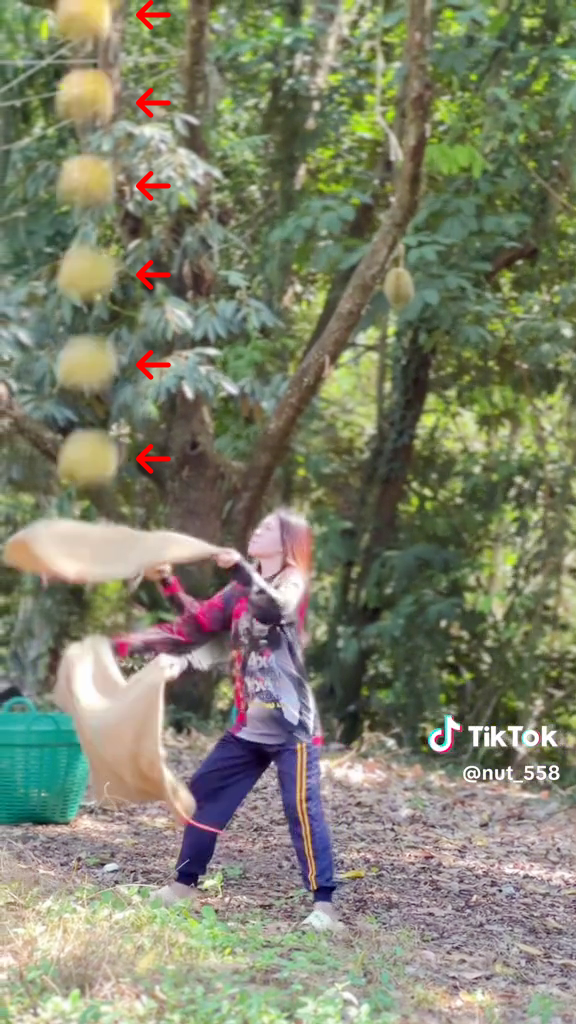
\includegraphics[height=2.5in]{images/Durian.png}
        \caption{}
    \end{subfigure}
    \caption{\label{fig:IntroApplications} The need to predict trajectories arises in many disciplines. (a) Close-In Weapon Systems (CIWS) are carefully designed by highly trained engineers to detect and neutralize airborne threats. \href{https://missiledefenseadvocacy.org/defense-systems/goalkeeper-close-in-weapons-system-ciws/}{https://missiledefenseadvocacy.org/defense-systems/goalkeeper-close-in-weapons-system-ciws/} (b) A highly evolved human worker predicts the trajectory of a falling durian fruit during harvest. \href{https://www.tiktok.com/@nut\_558}{https://www.tiktok.com/@nut\_558}}
\end{figure*}

Consider the phenomenon of an object flying through the air. A wide variety of applications depend on the ability to accurately predict the future location of such flying objects. Examples of automated computer systems tracking projectile objects are abundant in the fields of missile/drone guidance and missile/drone defense (Fig.~\ref{fig:IntroApplications}(a)). Beyond automated systems, human minds have to compute trajectories in many scenarios. Many sports require throwing and catching balls, and even in agriculture there is a need to predict trajectories (Fig.~\ref{fig:IntroApplications}(b)).

We're going to model an object traveling on a ballistic trajectory. We will take samples of the position of some object over time, then use those samples to fit a trajectory, then use that trajectory to predict where the object will impact the ground.

